\documentclass{standalone}
\usepackage{tikz,pgfplots,calc,tkz-euclide}
\usetikzlibrary{positioning,calc}
\usetikzlibrary{arrows}
\usepackage{tkz-euclide}
\usetkzobj{all}

\renewcommand{\familydefault}{\sfdefault}
\begin{document}
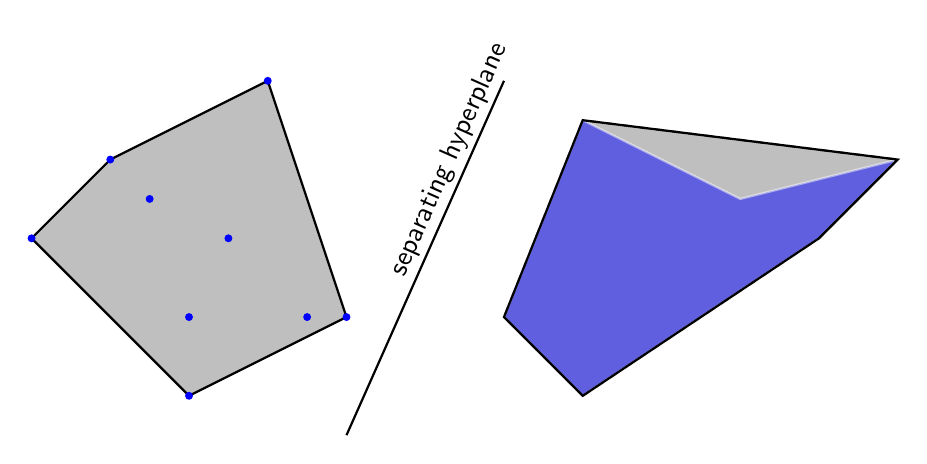
\begin{tikzpicture}[>=stealth, thick]
   
    % \def\a{1}
    % % \begin{scope}[xshift = 14cm, yshift = -3cm, scale = 1.7]
    %     % \draw[domain=-2:1.5,smooth,variable=\x,black] plot ({\x},{exp(\a*\x)});      
    %     \draw[domain=-2:3,smooth,variable=\x,black] plot ({\x},{.3*\x*\x});  


    %     \def\xx{-1}
    %     \def\xy{.3}    
    %     \def\yx{2.5}
    %     \def\yy{6.25*.3}
    %     \def\t{.4}
    %     \def\u{.6}
    %     \def\zx{{\t*\xx + \u*\yx}}
    %     \def\zx{1.1}
    %     \def\zy{{\t*\xy + \u*\yy}}
    %     \def\vy{{.3*\zx*\zx}}
    %     \def\vy{.35}


        \draw [fill = gray!50] (0, 0) -- (2, 1) -- (1, 4) -- (-1, 3) -- (-2, 2) -- cycle;
        \draw [fill = blue, draw = blue] (0, 0 ) circle (1pt);
        \draw [fill = blue, draw = blue] (2, 1 ) circle (1pt);
        \draw [fill = blue, draw = blue] (1, 4 ) circle (1pt);
        \draw [fill = blue, draw = blue] (-1, 3 ) circle (1pt);
        \draw [fill = blue, draw = blue] (-2, 2 ) circle (1pt);

        \draw [fill = blue, draw = blue] (.5, 2 ) circle (1pt);
        \draw [fill = blue, draw = blue] (1.5, 1 ) circle (1pt);
        \draw [fill = blue, draw = blue] (-.5, 2.5 ) circle (1pt);
        \draw [fill = blue, draw = blue] (0, 1) circle (1pt);


        \begin{scope}[xshift = 5cm]
            \draw [fill = gray, opacity = .5, dashed] (0, 0) -- (3, 2) -- (4, 3) -- (0, 3.5) -- (-1, 1) --cycle;
            \draw [fill = blue, opacity = .5, draw = white] (0, 0) -- (3, 2) -- (4, 3) -- (2, 2.5) -- (0, 3.5) -- (-1, 1) --cycle;
            \draw [] (0, 0) -- (3, 2) -- (4, 3) -- (0, 3.5) -- (-1, 1) --cycle;
        \end{scope}

        \draw (2, -.5) -- (4, 4);
        \node [rotate = 66] at (3.3, 3) {separating hyperplane};
        
\end{tikzpicture}
\end{document}